\documentclass[10pt,a4paper]{book}
\usepackage{graphicx}
\graphicspath{{figures/}}

\title{A Laboratory Course on Single Molecule Localization Microscopy}

\author{Kyle M. Douglass}

\date{\today}

\begin{document}

\maketitle

\chapter{Introduction}

\section{Learning Outcomes}

\begin{enumerate}
    \item Explain how a modern epifluorescence microscope works, including a list of its main components and their relationships to one another.
    \item Identify the main components of an epifluorescence microscope on the real microscope in the lab.
    \item Explain the principle behind single molecule localization microscopy and how it overcomes the diffraction limit of light.
    \item Illustrate fluorescence phenomena using state diagrams.
    \item Analyze data from the microscope to produce super-resolved images of cellular structures.
\end{enumerate}

\chapter{The Modern Fluorescence Microscope}

\chapter{Single Molecule Localization Microscopy}

\chapter{Fluorescence Photophysics}

\chapter{Localization Microscopy in Practice}

\begin{figure}[ht]
    \centering
    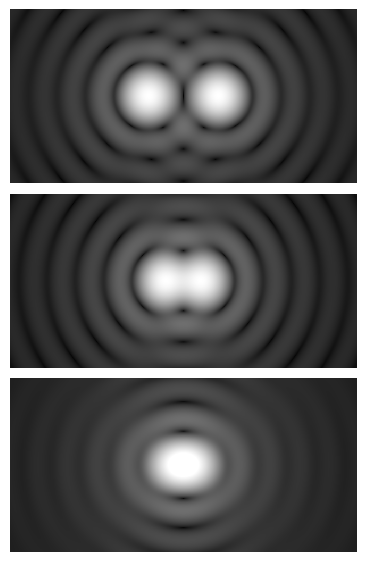
\includegraphics[width=0.75\textwidth]{Airy_disk_spacing_near_Rayleigh_criterion.png}
    \caption{Rayleigh criterion}
    \label{fig:rayleigh}
\end{figure}

\end{document}
